\documentclass[tikz,border=8pt]{standalone}
% Shared TikZ style for synorg platform diagrams. Each diagram \input's this
% inside a standalone document. Palette tracks the Material "teal" site theme so
% figures read as one system in light mode (SVGs are theme-neutral otherwise).
\usetikzlibrary{arrows.meta,positioning,shapes.geometric,fit,backgrounds,calc,decorations.pathreplacing}

\definecolor{synteal}{HTML}{00897B}   % primary
\definecolor{synfill}{HTML}{E0F2F1}   % light fill
\definecolor{synamber}{HTML}{B26A00}  % warning / lend
\definecolor{synred}{HTML}{B00020}    % deny / danger
\definecolor{syngrey}{HTML}{5F6368}   % muted

\tikzset{
  >=Stealth,
  font=\sffamily\small,
  box/.style={draw=synteal,line width=0.6pt,rounded corners=2pt,fill=synfill,
              inner sep=5pt,align=center},
  plane/.style={draw=synteal,line width=0.8pt,rounded corners=3pt,fill=synfill,
                inner sep=8pt,align=center},
  state/.style={draw=synteal,line width=0.7pt,circle,fill=synfill,inner sep=3pt,
                minimum size=11mm,align=center,font=\sffamily\footnotesize},
  decision/.style={draw=synteal,line width=0.7pt,diamond,aspect=2,fill=synfill,
                   inner sep=1pt,align=center,font=\sffamily\footnotesize},
  deny/.style={draw=synred,fill=synred!8,text=synred},
  warn/.style={draw=synamber,fill=synamber!10},
  flow/.style={->,line width=0.6pt,draw=syngrey},
  flowlbl/.style={font=\sffamily\footnotesize,text=syngrey,inner sep=2pt},
  note/.style={font=\sffamily\footnotesize\itshape,text=syngrey},
}

\begin{document}
% Which tier a change lands in, derived from blast radius, not self-selected
% (capability-tiers.md). Each decision routes to one enforcement mechanism:
% admission hard-deny (never), required review (human-by-exception), or the
% make-validate merge gate (autonomous).
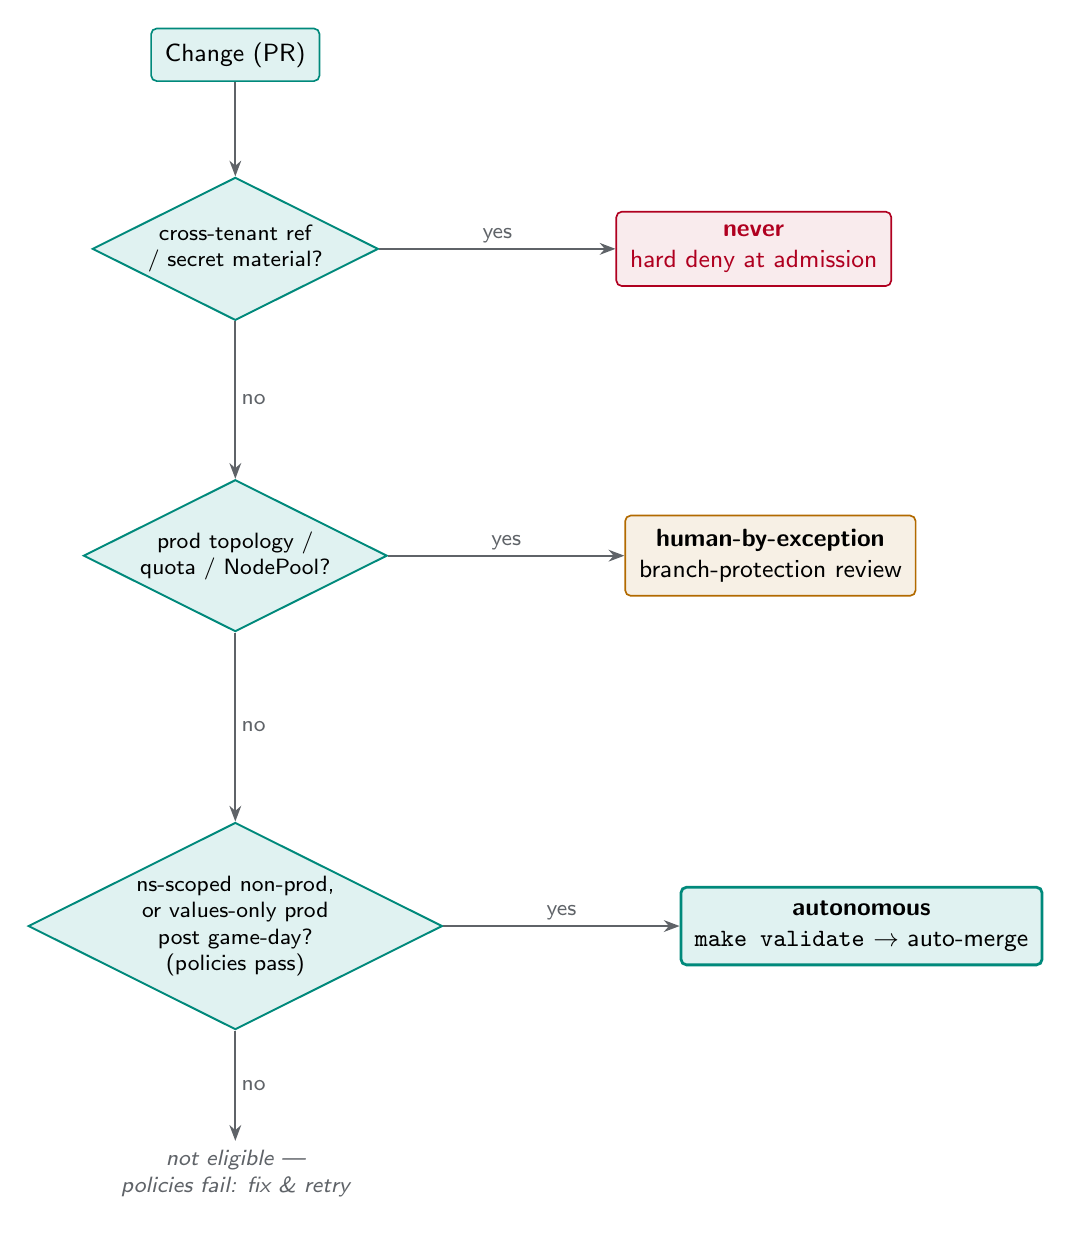
\begin{tikzpicture}[node distance=12mm and 30mm]
  \node[box] (pr) {Change (PR)};
  \node[decision,below=12mm of pr] (d1) {cross-tenant ref\\/ secret material?};
  \node[decision,below=20mm of d1] (d2) {prod topology /\\quota / NodePool?};
  \node[decision,below=24mm of d2] (d3) {ns-scoped non-prod,\\or values-only prod\\post game-day?\\(policies pass)};

  % outcomes (right column), one per enforcement mechanism
  \node[box,deny,right=of d1] (never)
    {\textbf{never}\\hard deny at admission};
  \node[box,warn,right=of d2] (human)
    {\textbf{human-by-exception}\\branch-protection review};
  \node[box,right=of d3,line width=1pt] (auto)
    {\textbf{autonomous}\\\texttt{make validate} $\to$ auto-merge};
  \node[note,below=14mm of d3,align=center] (retry)
    {not eligible ---\\policies fail: fix \& retry};

  \draw[flow] (pr) -- (d1);
  \draw[flow] (d1) -- node[flowlbl,above]{yes} (never);
  \draw[flow] (d1) -- node[flowlbl,right]{no} (d2);
  \draw[flow] (d2) -- node[flowlbl,above]{yes} (human);
  \draw[flow] (d2) -- node[flowlbl,right]{no} (d3);
  \draw[flow] (d3) -- node[flowlbl,above]{yes} (auto);
  \draw[flow] (d3) -- node[flowlbl,right]{no} (retry);
\end{tikzpicture}
\end{document}
